\section{Introduction}\label{sec:intro}


%Notes on wording 

% If we define entropy as complexity in the paper (as we do currently) we could say that every signal complicated or not has a balance between temporal/predictive structure and complexity (entropy). So for example, a chaotic signal and a random walk signal are both "complicated" they exhibit interesting behavior (they aren't monotonic, periodic, constant etc.) but one of them is far more complex and less predictable than the other , e.g.,  a random walk or gcc for example is complicated *and* highly complex (very high entropy) where as col is also complicated but not as complex as it exhibits a great deal of predictive structure (low entropy).

%An interesting contribution here is that examining a complicated signal (i.e., something that has interesting behavior, not periodic, monotonic, constant etc) of noisy real-valued entries, it is hard to determine a priori (without WPE) where in the spectrum of temporal structure and complexity the signal lies. Is it completely complex and have little to no predictive structure e.g., gcc or is it balanced in complexity and structure like a chaotic signal e.g., col.

%One potential issue here is that apparently information %theorists say that completely random signals are void of complexity. So Saying that a random walk signal (i.e., a signal with high entropy) is complex may cause some issues. HOWEVER, if we define complexity as entropy I don't think this is an issue. 

%Ryan does this seem reasonable? Is this an accurate synopsis of our discussion. Please feel free to add to it. Liz do you think making this distinction between "Complicated" and "Complex" would be useful for the readers understanding and dissemination of this topic?

%This would suggest changing the title to something a long the lines of "Decoding Complicated Time Series: The balance between complexity and temporal structure and the implications for predictability "



BRAINSTORMING 
\begin{itemize}
\item Complexity need not be hard to predict (can point at the simple predictions paper) [[move to introduction]]
\item random walk for example is best predicted by guess what just happend[[move to introduction]]
\item The kind of complexity present matters, i.e., that is whether the complexity is structured or not.[[use here and mention in intro]] 






\item \col brings about the point nicely that some prediction strategies cannot utilize the processes internal information transfer method. That is a nonlinear internal information transfer system cannot be predicted effectively with a linear strategy. This gives a practitioner leverage on when to give up and when to keep working. [[use in this section as bridge to next section]]

\end{itemize}



%\begin{it}
%Paragraph on computer performance, including citations to Todd paper
%and summary of the results that indicate that they're deterministic
%nonlinear dynamical systems.  Given that, we should be able to
%predict.  What benefits would accrue if we could do so: power mgmt,
%end world hunger [[this is my primary goal everyday :)]], etc.
%\end{it}
Things to add to introduction
\begin{enumerate}
\item Different kinds of complexity exist in time series and this makes choosing prediction models difficult 
\subitem NOTE: RW and chaos are both complex. One is predictable and one is not.

\item Make an argument that Computer Performance is a great testing ground as it omits signals that completely cover the spectrum of complexity \col \dots \gcc

\item When deterministic structure even complex structure exists that structure can be utilized for prediction. 
\item For noisy real-valued time series distinguishing randomness (WN,RW) complexity from structured nonlinear / chaotic /high period / high dimensional etc complexity is (until now) very hard. 
\subitem for this provide predictions of \gcc and \col side by side and discuss "How can we tell if we did a bad job because the method is inadequate vs the signal being too complex. Lead this into is it possible to tell if there exists structure in a time series to know if we should find a better model or not. Maybe even having 4 predictions. top being ARIMA of the above signals and bottom being LMA of the above signals. Show that one improved and one did not. Is it that we used the wrong method to predict or is it that we simply can't predict the signal better than a random walk due to high levels of internal signal complexity.



\item Introduce the two main contributions of the paper which are outlined at the begining of the results section

\end{enumerate}
\noindent ***NOTES END HERE****

\noindent ****SECTION START****


Complicated time series are ubiquitous in modern scientific research. 
%Characterizing and forecasting the future behavior of these observed systems is a vastly researched area with many open questions. 
Every observed time series, complicated or not, exists on a spectrum of \emph{complexity}\footnote{An approx of (blah ) entropy which we make more rigorous in blah}. On the low end of that spectrum are time series that exhibit perfect predictive structure, i.e, signals whose future value are perfectly predicted by knowledge of past values from some ``ideal" model. In particular, there is a an underlying process that generates and transmits information from the past to the future in a perfectly predictable fashion. Some examples of this are constant or low-period signals. On the opposite end of this spectrum are signals which are ``fully complex", i.e., the underlying generating process creates information so rapidly that no information at all is transmitted from the past to the future. Some examples, of this are white noise or random walk processes. With signals on this side of the spectrum, knowledge of the past gives absolutely no insight into the future, \emph{regardless} of the chosen model.  In the middle of this spectrum are where complicated \emph{and} forecast-able signals exist, e.g., deterministic chaotic trajectories, high period signals with some level of noise on top. With time series in this portion of the spectrum, enough information is being transmitted from the past to the future that given the \emph{ideal} model the future of the observed system could be forecast with high accuracy. 

Unfortunately, as a corollary of the undecidability of the halting problem: there cannot exist \emph{one} universally ideal forecasting scheme for even completely noise-free deterministic time series\cite{weigend-book}, let alone an arbitrary time series. This naturally leads to an important and hard question: given a complicated real-valued time series, is it possible to reliably quantify where on this spectrum the time series lies? That is, when little or nothing is known about the underlying system's generating process (e.g., linear, nonlinear, deterministic, stochastic, stationary, non-stationary etc.) how can we infer from a noisy real-valued time series if the signal is too \emph{complex} to forecast?






To answer this question and for the purposes of this paper we focus on real-valued (possibly) noisy scalar time series which appear \emph{complicated}, i.e., they exhibit interesting behavior, for instance, not of low period, strictly monotonic, or constant. We make no assumptions about the generating process's properties,(e.g., linear, nonlinear, deterministic, stochastic, stationary, non-stationary, etc.) and we attempt to measure empirically where on the previously mentioned spectrum of \emph{complexity} the time series exists.
We argue that \emph{permutation entropy}
\cite{bandt2002per}, a method for measuring the entropy of a
real-valued-finite-length noisy time series through ordinal analysis, is an effective way to explore that conjecture. For the purposes of this paper we define complexity as \emph{permutation entropy}, which we define and explain rigorously in Section \ref{sec:meaComplex}.  To validate these claims we model the time series using a variety of forecasting models which we introduce in Section \ref{sec:model}. We then compare the empirically estimated \emph{complexity} with the accuracy of each forecast method. Which results in two primary findings:


\begin{enumerate}

\item The complexity of a noisy real-valued time series is quantifiable.

\item The way information is processed internally by a given process plays a crucial role in the success of different forecasting schema.

\end{enumerate}






%[[Introduce and make it clear why we choose comp. perf. as test bed.]]
[[Move this up]]
To explore this conjecture we require a test bed for generating a broad array of time series to analyze which covers the full spectrum of complexity. We argue that the ideal test bed for this purpose is computer performance. Computers are among the most complex engineered artifacts in current
use.  Modern microprocessor chips contain multiple processing units
and multi-layer memories, for instance, and they use complicated
hardware/software strategies to move data and threads of computation
across those resources.  These features---along with all the others
that go into the design of these chips---make the patterns of their
processor loads highly complicated. Accurate forecasts of these quantities, if one could
construct them, could be used to improve computer design. 
% If one
%could predict that a particular computational thread %would be bogged
%down for the next 0.6 seconds waiting for data from main memory, for
%instance, one could save power by putting that thread %on hold for that
%time period (e.g., by migrating it to a processing %unit whose clock
%speed is scaled back). 
 Computer performance traces are, however, very
complicated and range across the entire spectrum of complexity, making this an ideal test bed.  Even a simple ``microkernel,'' like a three-line loop that
repeatedly initializes a matrix in column-major order, can produce everything from periodic to
{\sl chaotic} performance traces \cite{mytkowicz09}, depending on the architecture running the software. Such a performance trace is shown in
Figure~\ref{fig:ipc}.%, and chaos places fundamental limits on predictability.
%
 \begin{figure}[htbp]
    \centering
    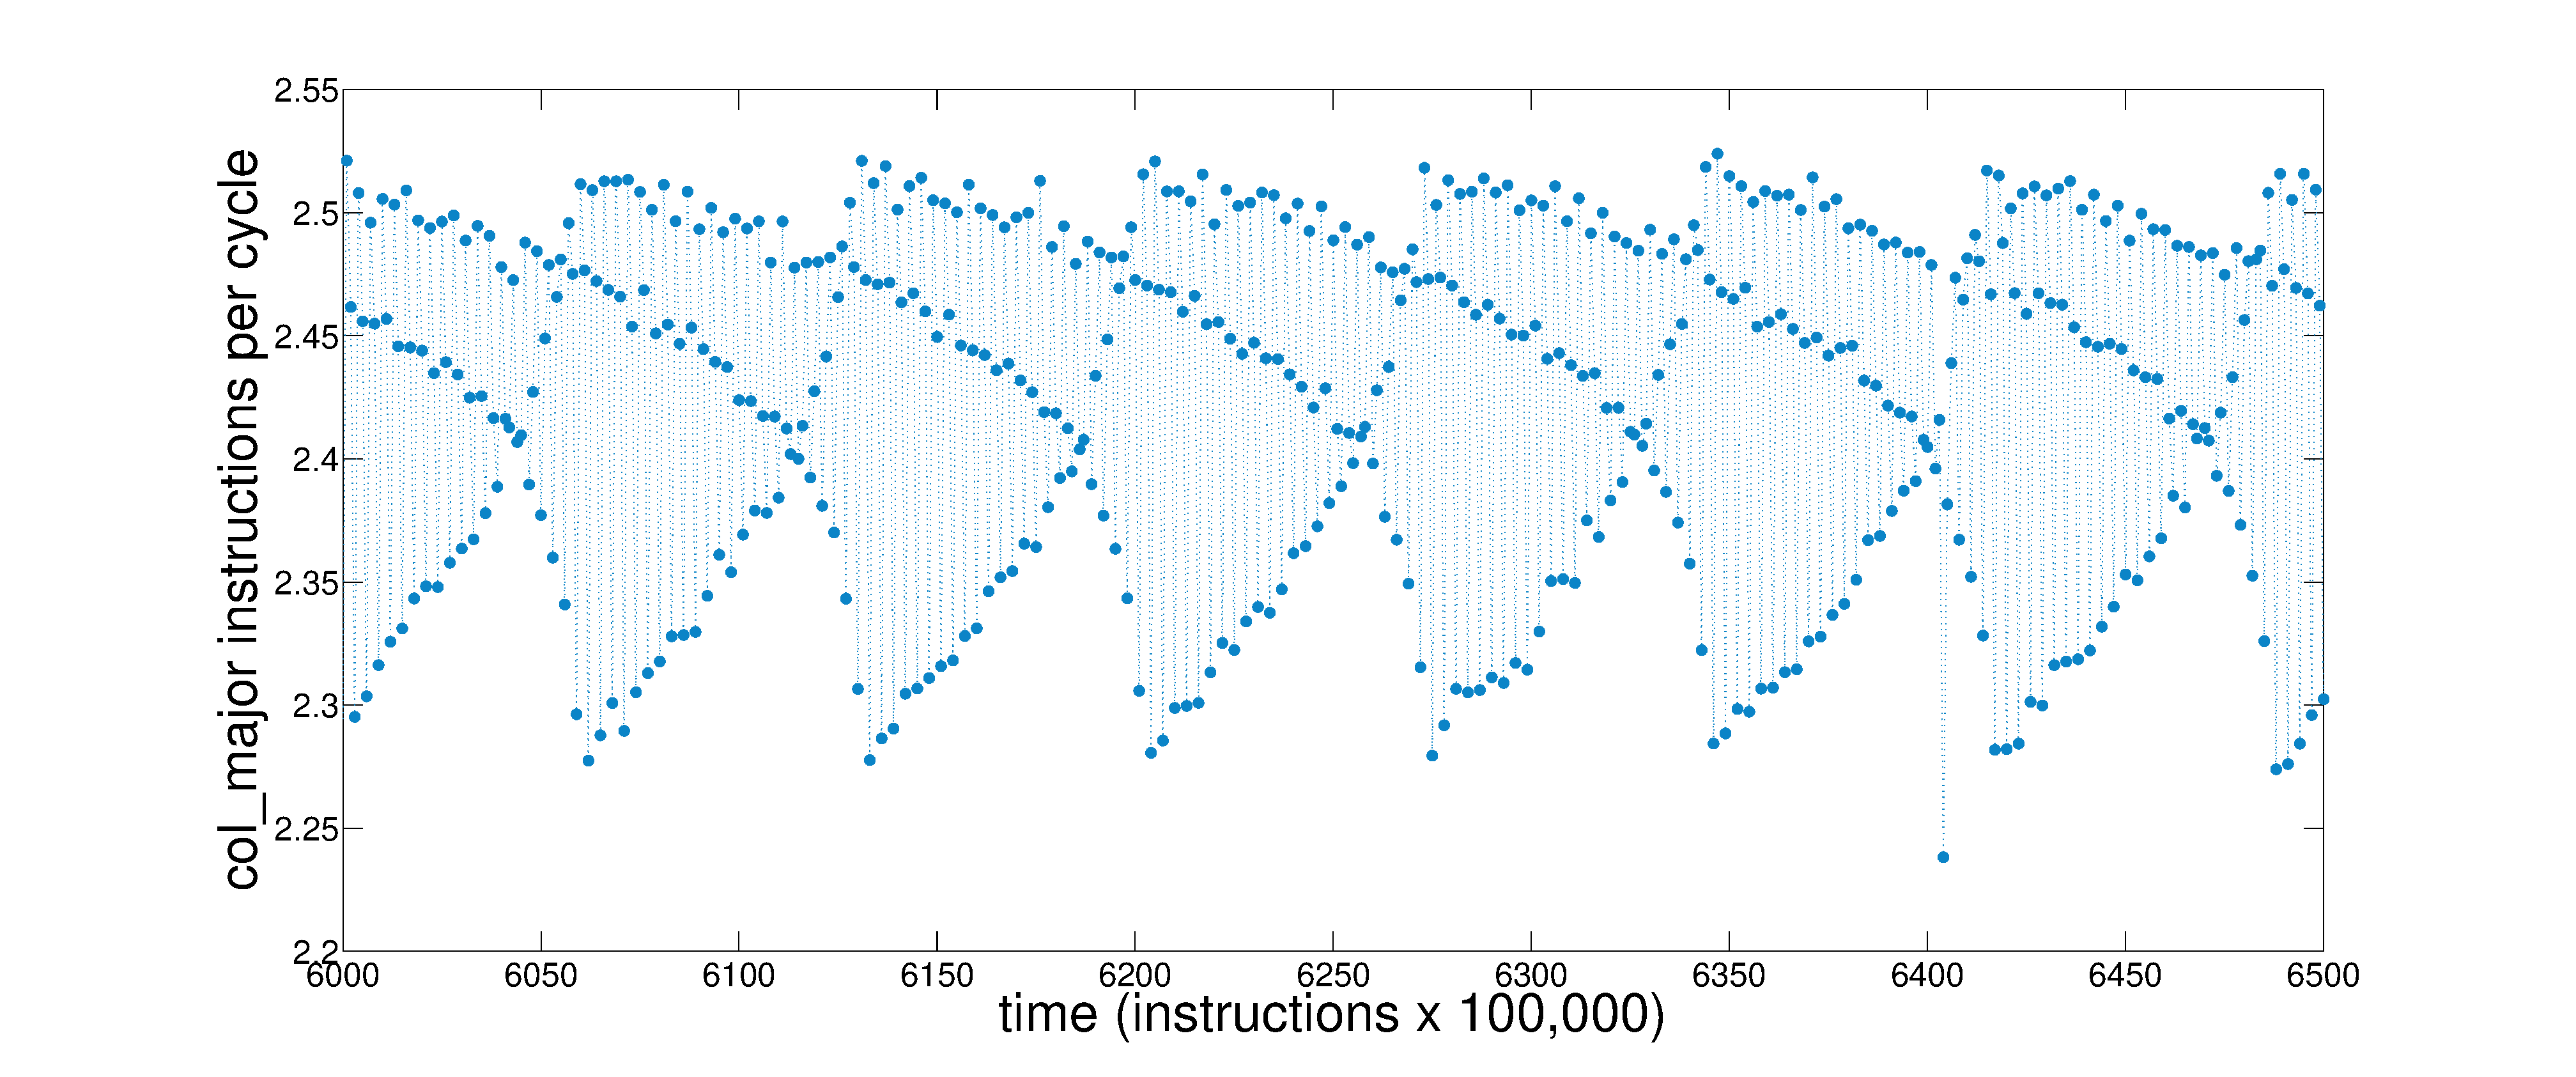
\includegraphics[width=\textwidth]{figs/colshortts}
    % where an .eps filename suffix will be assumed under latex,
    % and a .pdf suffix will be assumed for pdflatex
    \caption{A small snippet of the instructions per cycle(ipc) of {\tt
        \col}, a three-line C program that repeatedly initializes
      a matrix in column-major order, running on an Intel i7\textsuperscript{\textregistered}-based machine.  Even this
      simple program exhibits chaotic performance dynamics.}
   \label{fig:ipc}
  \end{figure}
With a single system producing complicated time series that vary so greatly in complexity, it would be invaluable to known a priori if a trace contained enough predictive structure to forecast before time and effort was spent on trying to model and forecast it. 

The computer systems community has applied a variety of prediction
strategies to traces like this, most of which employ regression.  An
appealing alternative builds on the recently established fact that
computers can be effectively modeled as deterministic nonlinear
dynamical systems \cite{mytkowicz09}.  This result implies the
existence of a deterministic forecast rule for those dynamics.  In
particular, one can use \emph{delay-coordinate embedding} to
reconstruct the underlying dynamics of computer performance, then use
the resulting model to forecast the future values of computer
performance metrics such as memory or processor loads
\cite{josh-ida2011}.  In the case of simple microkernels like the one
that produced the trace in Figure~\ref{fig:ipc}, this deterministic
modeling and forecast strategy works very well.  In more-complicated
programs, however, such as numerical software or compilers,
this forecast strategy---as well as the traditional methods---break
down some of the time, but work fine others.

This paper is a first step in understanding when, why, and how
deterministic forecast strategies fail when they are applied to
deterministic systems.  We focus here on the specific example of
computer performance but believe the results apply to a much broader class of time series.  We conjecture that the complexity of traces
from these systems---which results from the inherent dimension,
non-linearity, and non-stationarity of the dynamics, as well as from
measurement issues like noise, aggregation, and finite data
length---can make those deterministic signals \emph{effectively}
unpredictable.  We argue that \emph{permutation entropy}
\cite{bandt2002per}, a method for measuring the entropy of a
real-valued-finite-length time series through ordinal analysis, is an
effective way to explore that conjecture.  We study three
examples---a simple microkernel and two complex programs: one from the
SPEC 2006CPU benchmark suite, and one from LAPACK---running on an Intel i7-based machine.  For
each program, we calculate the permutation entropy of the processor
load (instructions per cycle), then compare that to the prediction accuracy attainable for
that trace using a series of deterministic models.

% paragraph to appease the theoretician in me
It is worth taking a moment to consider the theoretical possibility of
this task. We are not attempting to predict the state of the CPU at an
arbitrary point in the future --- this, at least with perfect
accuracy, would be tantamount to solving the halting problem. What we
are attempting is to predict aspects or functions of the running of
the CPU: instructions executed per second, cache misses per 100,000
instructions, and similar statistics. Prediction of these quantities
at some finite time in the future, even with perfect accuracy, does
not violate the Rice-Shapiro theorem.

 The rest of the paper is organized as follows.
 Section~\ref{sec:compModel} describes the experimental setup, as well
 as the nonlinear modeling and forecast strategies.  In
 Section~\ref{sec:meaComplex}, we review permutation entropy, calculate
 its value for a number of different computer performance traces, and
 compare the results to the prediction accuracy.  In
 Section~\ref{sec:conc}, we discuss these results and their
 implications in regard to our conjecture, and consider future areas of
 research.

